\documentclass[UTF8,a5paper,10pt]{ctexbook}

\usepackage[utf8]{inputenc}
% \usepackage{ctex} %导入中文包
\usepackage{geometry} %设置页边距的包
\usepackage{enumitem}
\usepackage{graphicx}
\usepackage{pdfpages} %本文最重要的一个包,就是将PDF文件加入到封面位置
\usepackage{ulem}
\newcommand{\code}[1]{\texttt{#1}}
\makeatletter
\renewcommand\tableofcontents{%
    \thispagestyle{empty}
    \section*{\contentsname
        \@mkboth{%
           \MakeUppercase\contentsname}{\MakeUppercase\contentsname}}%
    \@starttoc{toc}%
    \newpage
    }

\geometry{left=2.5cm,right=2cm,top=2.54cm,bottom=2.54cm} %设置书籍的页边距

\title{大学计算机基础(理科)Python实用手册}
\author{Dill Chu编著}

\begin{document}
\section*{前言}
\addcontentsline{toc}{chapter}{前言}
\pagenumbering{roman}
\setcounter{page}{1}

大学计算机基础课程是计算机学院承担教学任务,
在北航学院托管开设的信息大类基础课程之一,是全体理科大类及强基计划,拔尖计划相关专业的学生在大一时应当修习的一门基础课程。
课程主要内容涵盖{计算机组成原理},{Python基础语法},{程序控制结构},{算法基础},{图表绘制},{数据分析},{GUI设计}等内容。
课程内容丰富,基本涵盖了理科大类对口各专业
在未来使用计算机作为工具,在实际科研或工作中解决问题的需求,或是提供了较好的入门指导工作,可以培养学习者的计算思维和运用计算机解决具体问题的能力。无论是否有计算机使用经验,是否有程序编写或脚本编写经历,在学习本课程后
都将具有相应的能力。

具体的课程内容与任务方面。课程主要包括2次讨论课,10次课内实验和1个大作业,所有题目都是助教同学利用寒假时间全新准备的。具体内容见下。

两次讨论课主要的内容是对图论
(七桥问题等的理解,最短路径问题等),最优化问题(枚举法,匈牙利算法等)等特定,相对较为复杂的算法与模型的理解和应用,
由每个人独立思考,而后在小组内讨论并向全班汇报解决思路与方案,课后每个人需要形成\dotuline{\textbf{独立的实验报告}}。

课内实验是跟随理论课程授课内容,对理论课上所讲授的知识进行上机运用的过程环节。课内共有10次实验,课内实验难度不是很大,最最重要的是\dotuline{\textbf{独立完成}}(包括提交到平台上的代码和实验报告)。

具体实验安排如下:
\begin{enumerate}[itemsep=2pt,topsep=0pt,parsep=0pt,start=0]
    \setlength{\itemsep}{-0.1cm}
    \item Python编程环境的使用
    \item Python基本语法
    \item 程序控制结构与列表
    \item 问题的描述—基本数据结构(字符串,字典)
    \item 问题的描述—自定义数据结构(栈,队列)
    \item 基本算法设计与实现(枚举,递归)
    \item 较复杂算法设计与实现(贪心法,动态规划)
    \item Python实现数据图形绘制
    \item 插值,拟合计算
    \item Pandas数据分析与GUI设计
\end{enumerate}
其中,前几次实验(实验0-实验2)的难点在于对Python最基础的语法的理解与运用,难在入门。这些内容并不是很难,甚至可以称得上非常简单。只是可能较为新鲜,此前没有接触过,才会带来一定的困扰。
只要实际上手写过一两个程序,这部分内容就可以很轻松地掌握。

在基础数据结构和算法部分(实验3-实验6),对知识本身的理解与运用则会成为相对困难的内容,但本课程的目的在于
培养运用与实用的思维,并不在于要求对这些算法有多么深刻的理解,也不会要求大家去leetcode等算法训练平台做大量的题来理解和巩固,当然,少量做一些题目,来提高和巩固自己也是欢迎的。
事实上,贪心法和动态规划都是计算机科学发展到现在,称得上是最基本,最简单而常用的计算机算法了,所以其难度并不是那么大,还请大家多多尝试学习和理解。

最后的几次实验(实验7-实验9),我认为这些是应用性较强的实验。直白来说,在这部分实验中,你并不需要知道多少原理,你要做的只是拿来几个模板,照猫画虎,按部就班地搭建“积木”,完成任务就可以了,并没有多少难度。
但鉴于Python是一门脚本语言,从笔者的实际经历来看,这些内容
在未来的实际科研和应用中,反而是非常非常有用的。

大作业通常在学期中后段布置,是一组具有不同难度系数,面向不同实用场景的实际问题的,较为系统和工程化的解决方案,是对整个学期课程所学的一次总体性的应用。在完成大作业的过程中,
往往需要跟随实验指导,自学一定量的知识。大作业题目具有一定的复杂性,所以也需要投入一定的时间去完成。通常在大作业后也会安排申优答辩环节,可以选择参加,需要花费一定的时间和精力去准备。

完成对课程内容和总体任务的介绍后,让我们回到编篡手册的目的上来。正如前面所说,本课程授课过程面临时间紧,任务重的困难,对于少部分没有计算机基础或使用经验的同学来说,学习这门课程的过程中可能会面临较大的困难。这往往体现在开展实验实操时进度不佳,或面对的困难较多而疲于应对。
而苦于授课教师和助教精力有限,分身乏术,在提供实验指导方面可能会有覆盖不到的地方,对部分同学的学习带来一定的压力,甚至是阻力。同时,实际线下实验指导时我们通常以口述方式进行指导,难以在讲述过程中配合相应的代码,最好的情况也是
配合同学当前所写的代码进行辅导。但这对描述问题和思路上时不利的。通常,配合代码示例的形式对问题和思路进行描述往往可以使读者(或者听众)对问题和思路形成更好的理解。
因此,我选择编篡本手册,一方面,是可以让同学们在每次实际进行实验前,通过学习实际题目和
代码的方式,能够能对这一部分的内容做大致了解,做到“手上有枪”;另一方面,我作为课程的修习者,以学生的视角编篡一份手册,
也是让大家能有一个相较于教材来讲,方便速查思路的材料。教材上的内容非常全面,高屋建瓴,但对于速查还是带来一定的困难,与同学们学习的思路上也不一定完全一致,而同龄人之间总是更容易找到相同的思路,产生一些共鸣。
\newpage
\tableofcontents
\thispagestyle{empty}
本书中所有代码,在Windows 11 23H2及macOS 14.2.1 23C71 arm64上以Anaconda 23.11.0, Python 3.11作为环境运行测试通过。具体第三方库版本见下:
\begin{enumerate}
    \item scipy
    \item numpy
    \item matplotlib
    \item pandas
\end{enumerate}
\newpage
\pagenumbering{arabic}
\chapter{Python编辑及运行环境}
在本课程中,我们选择安装anaconda这一Python发行版进行学习与开发。一方面是因为anaconda在安装时不仅仅能够安装一个python解释器,
其也会同时安装IPython kernel,Jupyter notebook,matplotlib,scipy,numpy等多个常用的(也就是本课程中会用到的)第三方库。另一方面,anaconda提供Spyder这一高集成度,
便于初学者学习和调试的IDE,可以提供给我们“开箱即用”的体验\footnote{anaconda本身也提供很多别的功能,本章节后面会进行简要介绍}。

如果你想要挑战自己,当然可以自行到Python项目官网\footnote{https://python.org}上自行下载和安装Python解释器,而后使用pip包管理工具安装
我们所需的各类第三方库或者第三方组件(包括Spyder,也可以通过pip来自动安装)。但在正式开始教程之前,需要强调,作为初学者,请不要同时安装
纯净Python解释器和anaconda,即不要
让使用下载的Python安装包所安装的python解释器同anaconda在同一台电脑上并存,因为此时你的电脑里将同时有两个python运行环境,且这两个运
行环境没有通过环境管理器进行管理,其激活次序,即运行python脚本文件时正在使用的python解释器,或是尝试使用pip安装第三方库所指向的环境不易明确。
总之,作为课程的初学者,也是本手册后面的安排,我们将基于anaconda(conda+python解释器)进行介绍,包括环境配置,工具使用等,
所有代码也将会在这个环境下进行运行。

本章节,我们将会介绍Anaconda的下载与安装过程,Spyder的基本使用方法,并在最后简要介绍conda环境管理工具和pip包管理工具的使用。
\section{Anaconda的下载与安装}
\subsection{Anaconda下载与安装}
Anaconda现已实现完善的公司化运营,可以访问其网站下载Anaconda:

https://www.anaconda.com/download

但通常,出于下载速度的考量,我们选择使用校园网联合镜像站的方式下载Anaconda,这不仅仅可以提供更快的安装包下载速度,同时其分发的
安装包也会将其中的默认镜像站替换成自己的分发站点,从而提供更高的pip与conda下载与更新速度。提供镜像站的组织有很多,如清华大学TUNA协会,中国科学技术大学所等高校及高校学生组织
所提供的下载源,此处以清华大学TUNA协会提供的下载源为例。

访问https://mirrors.tuna.tsinghua.edu.cn/anaconda/archive/ \footnote{此为双栈站点,可以自动选择IPv4或IPv6解析,将mirrors替换为mirrors6则只解析IPv6,替换为mirrors4则只解析IPv4,在校园网环境下,使用IPv6下载的文件不计流量。},
获取anaconda安装包列表。根据自己的操作系统版本和硬件架构,选择
下载对应的安装包体(如Windows-x86\_64对应AMD,
Intel处理器的Windows设备,MacOSX-arm64对应搭载Apple Silicon M1、M2、M3的设备)。
在当前的时间节点,建议选择Anaconda3-2023.09开头的安装包。如图\ref{fig:anacondaSelection}所示
\begin{figure}[htbp]
    \centering
    \includegraphics*[width=0.8\linewidth]{pic/tuna_anacondaDownload.png}
    \caption{Anaconda3安装包示例}
    \label{fig:anacondaSelection}
\end{figure}

对于不太熟悉命令行操作的同学来说,建议下载文件拓展名为pkg或exe的安装包,其可以提供图形化的安装界面和选项。具体安装过程在此不再赘述,
但请注意,\textbf{不要}把Anaconda安装在\dotuline{含有中文的目录}下,尤其注意你的Windows用户名是否带有中文。如果你不确定,可以直接将其安装在C盘外的其
他盘符\footnote{不要将Anaconda安装在C:/Program Files中},另外创建的文件夹中。

\subsection{环境变量配置}
配置环境变量的目的是令其他程序在运行python时能够直接找到base环境下的python,而不需要手动指定,同时也方便我们直接打开命令行就可以直接使用python解释器运行和调试程序。
anaconda提供了方便快捷的命令行环境的环境变量配置方式,只需要切换到conda.exe的安装
位置\footnote{windows下的默认位置C:\textbackslash Users\textbackslash 用户名\textbackslash anaconda3\textbackslash Script,macOS下的默认位置/Users/用户名/anaconda3/bin},直接
在命令行中运行{\texttt{conda init}}即可\footnote{对于powershell,需要使用\texttt{.\textbackslash conda init}}。运行效果如图\ref{fig:condaInit}所示。
\begin{figure}[htbp]
    \begin{minipage}[t]{0.4\linewidth}
        \centering
        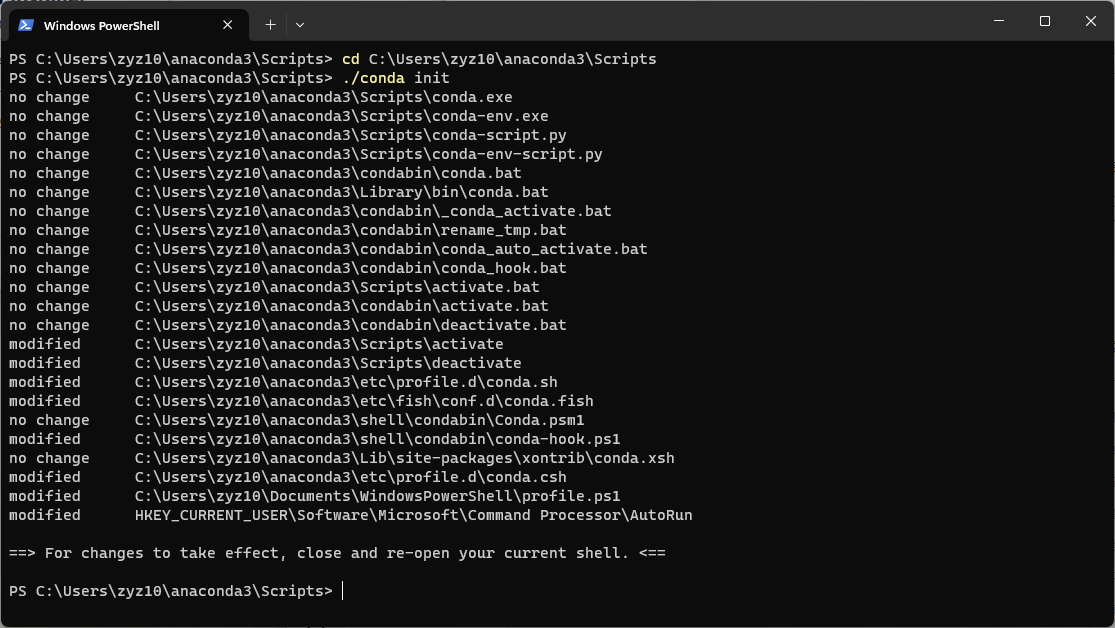
\includegraphics[height=0.5\linewidth]{pic/conda_init_windows.png}
        Windows
    \end{minipage}
    \hfill
    \begin{minipage}[t]{0.4\linewidth}
        \centering
        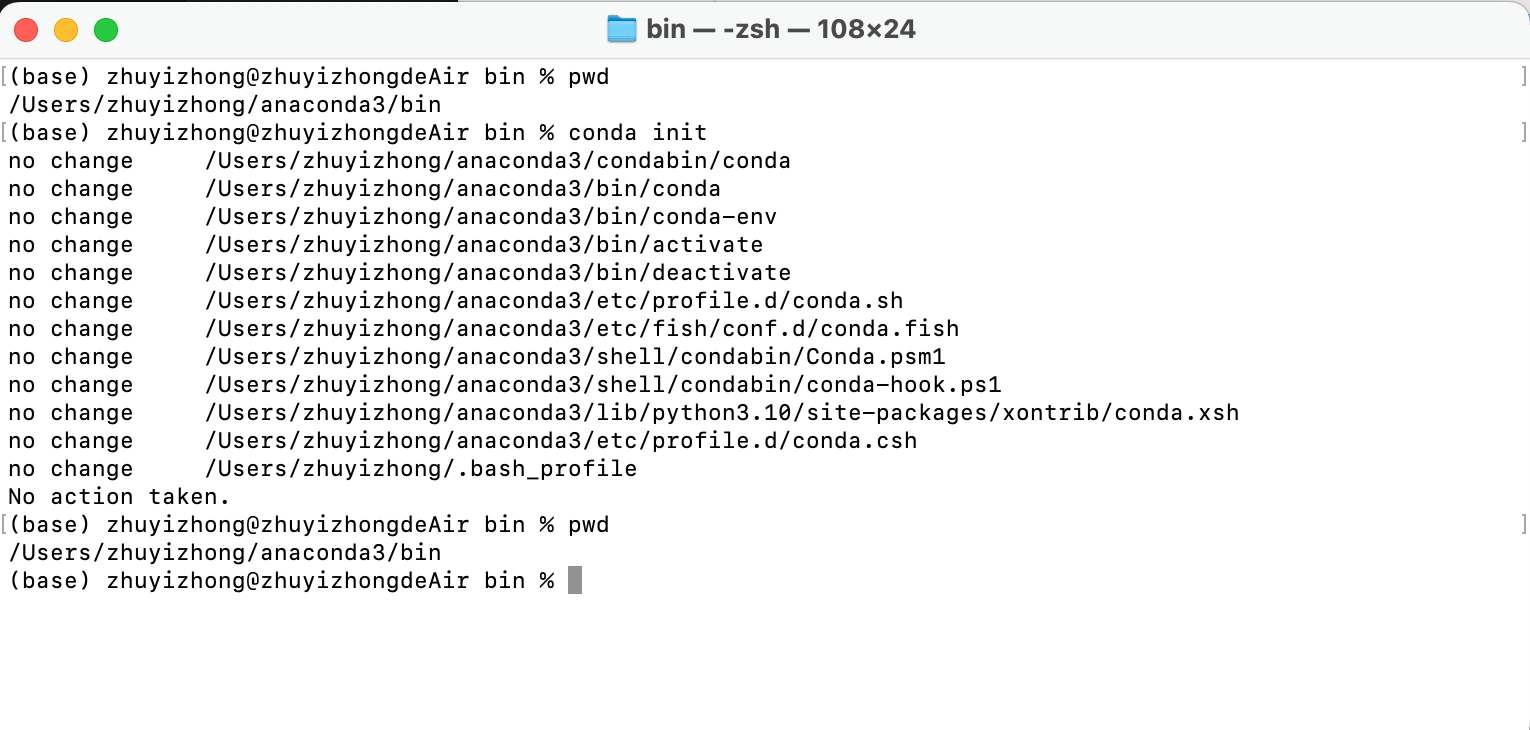
\includegraphics[height=0.5\linewidth]{pic/conda_init_macos.png}
        macOS
    \end{minipage}
    \hfill
    \caption{使用~conda init~自动配置环境变量的结果}
    \label{fig:condaInit}
\end{figure}

而后,重新打开命令行
(Windows 10/11中的终端\footnote{打开powershell时如果出现异常报错,则
需要使用Win+X点选终端(管理员)打开powershell,运行Set-Execution
Policy RemoteSigned以使能脚本运行功能},macOS中的控制台),可以看到在命令
前面出现了(base)字样,表明当前激活的python环境是conda管理的base环境。

至此,anaconda 的环境配置已经基本结束。对于 Windows 用户,如有需要,还可以在高级系统设置中
手动将 anaconda 安装目录下的 bin 和 Script 目录添加到 Path 中,在此不再赘述。今后的课程学习中,
用到的可能性很小。

\section{Spyder使用}
Spyder 是今后我们在课程学习上将要主要使用的 IDE\footnote{集成开发环境},也是考试时要用的考试机上
所具备的唯二的 Python 代码编辑工具\footnote{另一个是 Python 安装时会有的 IDLE,不具备联想提示和调试功能}。
Spyder 基于 IPython kernel 运行和调试 Python 代码,可以直观的将当前时刻各变量的值显示在窗口上,同时也具有
命令行窗口,方便直接运行指令进行测试,或对变量值进行直接的修改。总之,对于初学者而言,Spyder 是非常简单,易用
的 Python IDE。下面将会对Spyder的功能进行简单的介绍。

安装流程结束后,在开始菜单(macOS:启动台)中寻找到 Anaconda Navigater,点击运行。
加载结束后,可以打开Spyder,如图\ref{fig:navigater}所示
\begin{figure}[htbp]
    \centering
    \includegraphics*[width=0.7\linewidth]{pic/anaconda_nav_Spyder.jpg}
    \caption{Anaconda Navigater主界面}
    \label{fig:navigater}
\end{figure}

下面介绍Spyder主界面各面板的功能。但在开始之前,我们先来把Spyder的界面语言修改成中文。点选 
Tools-Preferences 打开选项页面,而后在Application-Advanced settings中找到Languages,选择简体中文即
可。如下图所示。
\begin{figure}[htbp]
    \begin{minipage}[h]{0.3\linewidth}
        \centering
        \includegraphics*[height=0.3\linewidth]{pic/Spyder_Language_1.png}
    \end{minipage}
    \hfill
    \begin{minipage}[h]{0.6\linewidth}
        \centering
        \includegraphics*[height=0.4\linewidth]{pic/Spyder_Language_2.png}
    \end{minipage}
\end{figure}
\newpage
下面介绍Spyder主界面各面板的功能与作用。设置中文并打开Spyder后,初始界面如图\ref{fig:spyderMain}所示。
\begin{figure}[htbp]
    \centering
    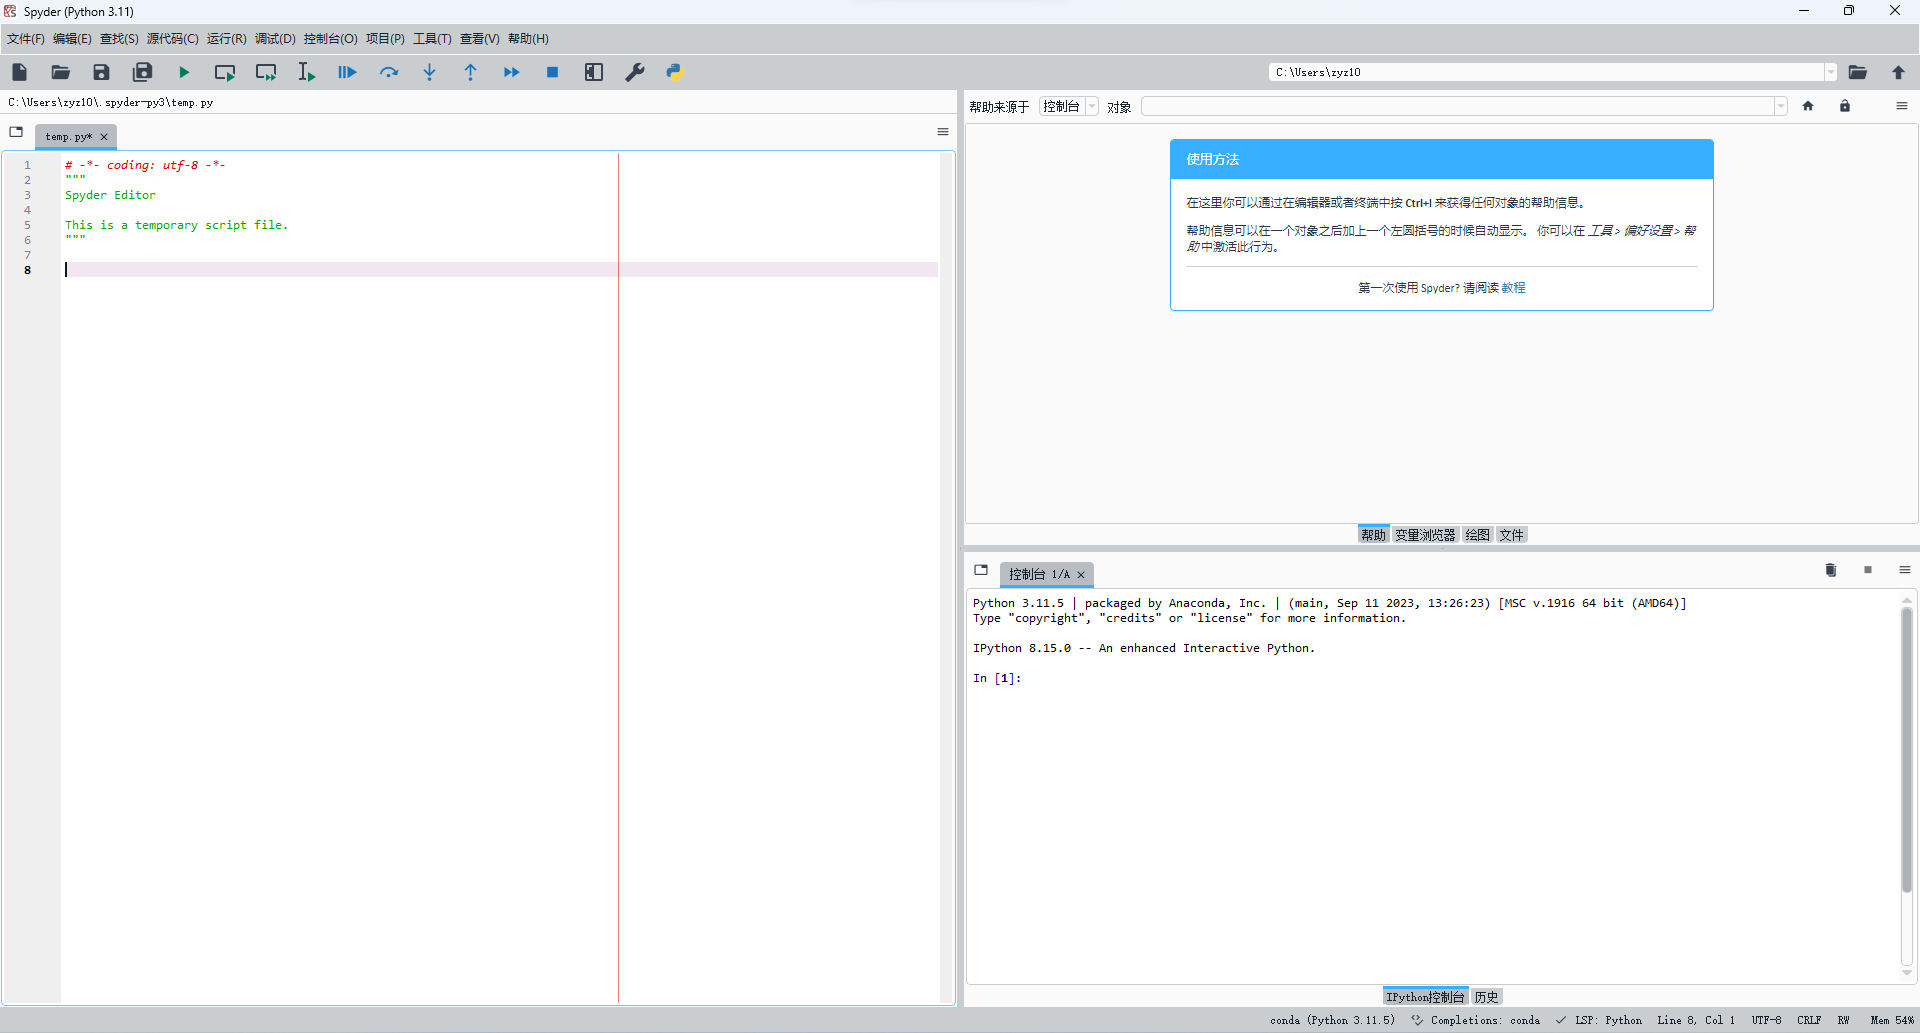
\includegraphics[width=0.7\linewidth]{pic/spyder主界面.png}
    \caption{Spyder 主界面}
    \label{fig:spyderMain}
\end{figure}
左侧是代码编辑区域,可以在此修改和编辑Python程序的源代码。可以看到在源代码编辑框右侧,未到达编辑框边界处有一根纵向的线,
这个位置代表 Python 源代码编写规范 PEP 8 中的要求,每行代码不超过79个字符。有兴趣的同学可以自行查找资料,深入了解 PEP 代
码规范。简单来说,PEP 8 是对代码可读性提供的规范,用来保证程序员书写出的代码具有可读性和可维护性。还请大家尽量遵循代码规范,
包括后面介绍基本语法时会提到的变量命名规范和注释规范等,方便各位同学后面再读懂自己的代码,也方便授课教师和我:-)。

右侧上半部分有Spyder提示,变量浏览器,绘图和文件四个选项卡。
Spyder提示可以显示库函数的帮助提示信息,具体使用方法在后面详细的语法部分将会进行更加详细的介绍。变量浏览器可以显示
当前内存中所存放的变量,包括类型、大小\footnote{可以理解为规模,如3x2的数组会显示为(3,2);普通的整形、浮点会显示为1}和值。
不同版本的Spyder在处理变量浏览器选项卡时可能有所不同,但总体上大同小异。我们只需要了解,双击值这一列对应的格子即可看到和修改
变量的值,便足够了。

绘图和文件选项卡在前期使用的较少。绘图选项卡可以保存每一次使用 matplotlib 等库绘制出来的图片,形成一个历史记录,方便查阅和调用。
具体使用方法将会在后面绘图的部分再行介绍。文件选项卡则会显示当前打开的 Python 文件所处的目录下面的文件,在后面进行文件操作
或处理大作业时,观察和操作当前目录下有哪些文件\footnote{包括其他 Python 脚本或者数据文件}非常便利。

右侧下半部分提供了一个命令行窗口,在此可以直接与 IPython 内核交互。Spyder 运行 Python 文件是使用 IPython 内核进行解释运行的,
如果真的直接使用 Python.exe 对文件进行解释运行,在每一次运行完程序之后,Python.exe 不会驻留在后台,相关内存会被释放,自然也
不能看到内存中存储的变量的情况。而原始的 Python 解释器也不提供调试功能。

书归正题,在这个命令行窗口中,我们可以直接创建变量,运行命令,抑或是在调试过程中修改变量的值,都是可行的。具体的使用方法,在下一章
将会结合具体代码进行概述。现在,你只需要了解到这个界面上各个块的功能即可。

再行补充一个知识,在命令行窗口右侧上部,可以看到一个三横线选项卡,将其打开,里面有对 IPython 内核的交互。如图 所示。可以新建,中断
或重启 IPython 内核。这对于程序陷入死循环或卡死时是十分有效的,可以在这里重启或直接开启一个新内核运行程序。当然,也可以直接关闭控制台
选项卡,这也能起到关掉对应 IPython 内核的作用,当没有 IPython 内核在运行时,Spyder 会自动开启一
个新的 IPython 内核\footnote{IPython中的I代表Interact,即交互。我一直将其称之为内核,其实其本质上就是一个进程,使用其运行 Python脚本,本质上就是
要求这个进程读取这个文件并进行解释运行。如果想要深入了解IPython,可以访问ipython.org}。
\begin{figure}[htbp]
    \centering
    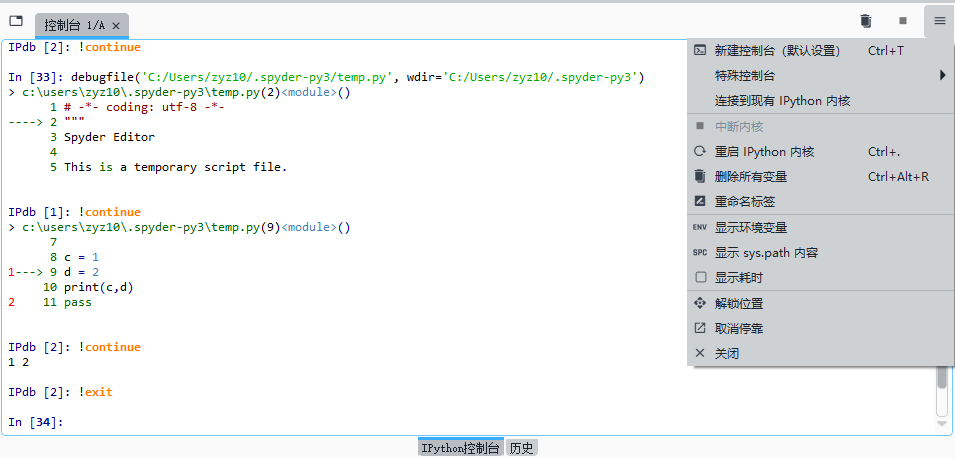
\includegraphics[width=0.8\linewidth]{pic/ipython_interact.png}
\end{figure}

\section{pip和conda的使用*}
在这一部分,我们将要介绍\texttt{pip}和\texttt{conda}的使用方法。这两个工具
都可以作为环境下的包管理工具,conda同时还可以作为虚拟环境的管理工具。在课程中,
我们使用这两个工具都不会特别深入,因此这里只介绍一些基础的使用方法。

\subsection{pip包管理工具}
Python 是一个具有系统性的包管理和共享体系的体系,pip 是python标准安装后会带有的包管理工具。
如果想要下载或使用一个第三方库,如matplotlib,scipy等,可以先访问https://pypi.org 查看包名,
文档和快速入门(如有)。也可以在这个平台上搜索第三方库。当搜索到一个第三方库后,可以使用下列格式的命令安装:
\lstset{language=bash}
\begin{lstlisting}
    pip install <package name> <-U> <-i> <mirror>
\end{lstlisting}
\texttt{package name}参数是必选参数,是包名。\texttt{<-i mirror>}参数是指定 \texttt{pip} 从哪个镜像站下载软件包,
\texttt{mirror}参数应当填写镜像站地址。比如下面这个例子
\begin{lstlisting}
    pip install scipy -U -i \
    https://pypi.tuna.tsinghua.edu.cn/simple
\end{lstlisting}
其指定使用清华大学 TUNA 协会的
镜像\footnote{另可参阅 TUNA 协会提供的 pypi 镜像使用
帮助:\\https://mirrors.tuna.tsinghua.edu.cn/help/pypi/},安装(以及升级)\texttt{scipy}库。
要补充说明的是,上面这个代码框内的“\textbackslash ”的目的只是为了换行使用,无论是 bash 还是 python 中,“\textbackslash ”符号
的含义均是将一行代码拆成两行书写,解释器会将第二行,甚至
更多行(如果你连续使用“\textbackslash ”的话)的内容按照顺序拼接到一起来理解和执行。

如果希望指定安装的库的版本,可以参考下面的示例:
\begin{lstlisting}
    pip install scipy==1.11.3
\end{lstlisting}
\subsection{conda环境管理工具}
anaconda 是 conda 管理工具的一个发行版,除此之外,还有 miniconda 等更加精简的发行版本,其更加适合于
诸如 Raspberry Pi 等资源相对有限的计算平台,以及运行在无头模式下的服务器上使用。本小节将集中于 conda 工具的
使用的介绍。

\subsubsection{conda创建和管理虚拟环境}
在安装完毕之后,anaconda会自动创建一个base环境,在本课程中,我们大部分情况下都可以在base环境内进行操作,这是因为我们
在课内所使用的第三方库的数量不是很多,集中在一个环境内进行操作不会带来什么问题。下面介绍一个可能的情况,在完成大作业时,
课程要求我们建立一个 GUI,假设你需要使用 PyQt6 (或者新版本的 PyQt5 )来建立你的GUI,这是一个非常好用的 GUI 库,而 Spyder 运行依赖
于特定版本的 PyQt5,二者会产生冲突。在这种情况下,创建一个新的虚拟环境便是必要的了。

下面介绍创建和管理虚拟环境的办法。conda 支持创建运行特定版本 python 的虚拟环境,如下所示:
\begin{lstlisting}
    conda create -n <name> python=<version>
\end{lstlisting}
\texttt{<name>}参数是虚拟环境的名称,支持大小写,且对大小写敏感。\texttt{<version>}是指定 python 解释器版本,
支持到小版本如3.10.3。可以观察下面的示例
\begin{lstlisting}
    conda create -n MyPythonSpace python=3.10.3
\end{lstlisting}
这里我们指定创建一个名为\texttt{MyPythonSpace}的虚拟环境,解释器版本为 3.10.3 。运行时
会提示是否继续,按下回车即为继续\footnote{形如\texttt{[y]/n}这样的确认提示,
在不输入任何字符的情况下直接回车,则默认值为y,若为\texttt{y/[n]},则默认值为n},运行输出如下:
\begin{lstlisting}
    Channels:
 - defaults
Platform: osx-arm64
Collecting package metadata (repodata.json): done
Solving environment: done

## Package Plan ##

  environment location: \
    /Users/<username>/anaconda3/envs/MyPythonSpace

  added / updated specs:
    - python=3.10.3


The following packages will be downloaded:

## 此部分为Python解释器包信息,略去 ##

The following NEW packages will be INSTALLED:

## 此部分忽略 ##


Proceed ([y]/n)? y


Downloading and Extracting Packages:
                                                                                                            
Preparing transaction: done
Verifying transaction: done
Executing transaction: done
#
# To activate this environment, use
#
#     $ conda activate MyPythonSpace
#
# To deactivate an active environment, use
#
#     $ conda deactivate

\end{lstlisting}
而后,运行\texttt{conda activate MyPythonSpace},即可激活\\\texttt{MyPythonSpace}虚拟环境,如下:
\begin{lstlisting}
(base) bin % conda activate MyPythonSpace
(MyPythonSpace) bin % python --version
Python 3.10.3
\end{lstlisting}
需要返回\texttt{base}环境时,只需要运行\texttt{conda deactivate}即可。

下面介绍使用conda对已有环境进行管理。首先,如果需要列出当前存在的所
有由conda管理的环境,可以运行\texttt{conda env list}。
其会列出当前存在的所有环境,以及其位置,如下列所示:
\begin{lstlisting}
# conda environments
#
base            /Users/username/anaconda3
MyPythonSpace   /Users/username/anaconda3/envs/MyPythonSpace
\end{lstlisting}
如需删除某环境,可以考虑运行:
\begin{lstlisting}
conda env remove --name <env>
\end{lstlisting}
如删除\texttt{MyPythonSpace}这一环境:
\begin{lstlisting}
conda env remove --name MyPythonSpace
\end{lstlisting}
这一命令可以删除这个Python环境下的所有软件包以及这个环境本身。

\subsubsection{使用conda进行包管理*}
下面介绍使用conda安装第三方库的一个示例。在大部分情况下,我们使用pip安装第三方库已经足够了,但在这里还是介绍一下。
同时,要注意,不要尝试使用pip管理conda安装的第三方库,反之亦然。

使用conda安装PyTorch的方法如下:
\begin{lstlisting}
    # From https://pytorch.org
    conda install pytorch::pytorch torchvision \
            torchaudio -c pytorch
\end{lstlisting}
运行之后,conda会在当前激活的虚拟环境下安装 pytorch, torchvision, torchaudio 三个第三方库。在这里,
\texttt{install}表明要求conda执行安装包的操作,\texttt{-c pytorch}指定在pytorch这一发行频道上查找
软件包。

如果需要卸载软件包,可以运行\texttt{conda remove --name <env> <package>}进行卸载软件包的操作。如,卸载\texttt{MyPythonSpace}中的\texttt{numpy}软件包:
\begin{lstlisting}
conda remove --name MyPythonSpace numpy
\end{lstlisting}

下面介绍使用conda对环境中的第三方库进行升级的方法。但需要注意的是,如果你的环境当前可以满足需求,不需要
用到新版本的特性,当前运行的版本也没有需要通过更新来修复的安全漏洞,那么就不要更新某个第三方库。同样的,
也不必对整个环境内的第三方库进行统一的更新,但在此仍然介绍这种方法。
\begin{lstlisting}
conda update --all
\end{lstlisting}
这样,conda便会更新当前激活的环境下的所有库。相似的,更新某个库的方法为:
\begin{lstlisting}
conda update <package>
\end{lstlisting}
\end{document}
